\documentclass[../main.tex]{subfiles} 
\usepackage{ctex}
\usepackage{xltxtra}
\usepackage{graphicx}
\usepackage{booktabs}
\usepackage{amsmath}
\usepackage{mathdots}
\usepackage{amssymb}
\usepackage{cite}
\usepackage{appendix}
\usepackage{array}
\usepackage{subfigure}
\begin{document}

    \subsection{相关系数法}

        \subsubsection{特征与标签之间的相关性}

            特征与标签之间的相关性利用corr函数检验每个特征与标签Transported的皮尔森相关系数。
            皮尔森相关系数也称皮尔森积矩相关系数,是一种线性相关系数,是最常用的一种相关系数。反映两个变量X和Y的线性相关程度,值介于-1到1之间,绝对值越大表明相关性越强。
            计算结果如图30所示。

            \begin{figure}[H]
                \centering
                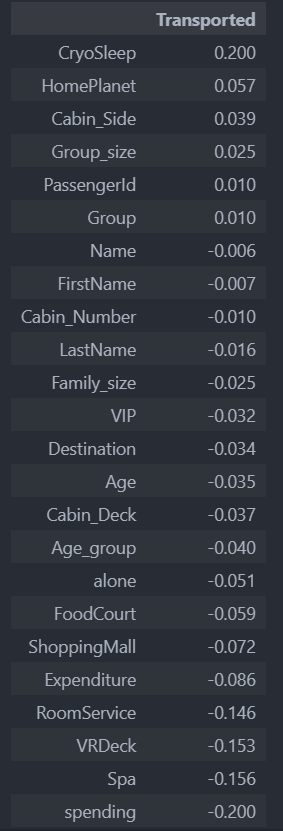
\includegraphics[scale=0.5]{Sec4_1.png}
                \caption{Pearson product-moment correlation coefficient}
            \end{figure}

            从图中我们可以看出,除了CryoSleep和spending特征与标签的相关性较强,其余很多特征与标签的皮尔森相关系数的绝对值甚至没有0.1,这无疑增加了模型学习的难度。
            其中Group\_Size、PassengerId、Group、Name、FirstName、Cabin\_Number、LastName、Family\_size这几个特征与标签的相关性甚至小于0.025,因此后续在数据选择的过程中可以考虑是否丢弃这几个特征。

        \subsubsection{特征与特征之间的相关性}

            两两计算特征之间的皮尔森相关系数并利用热力图对结果进行可视化,如图31所示。

            \begin{figure}[H]
                \centering
                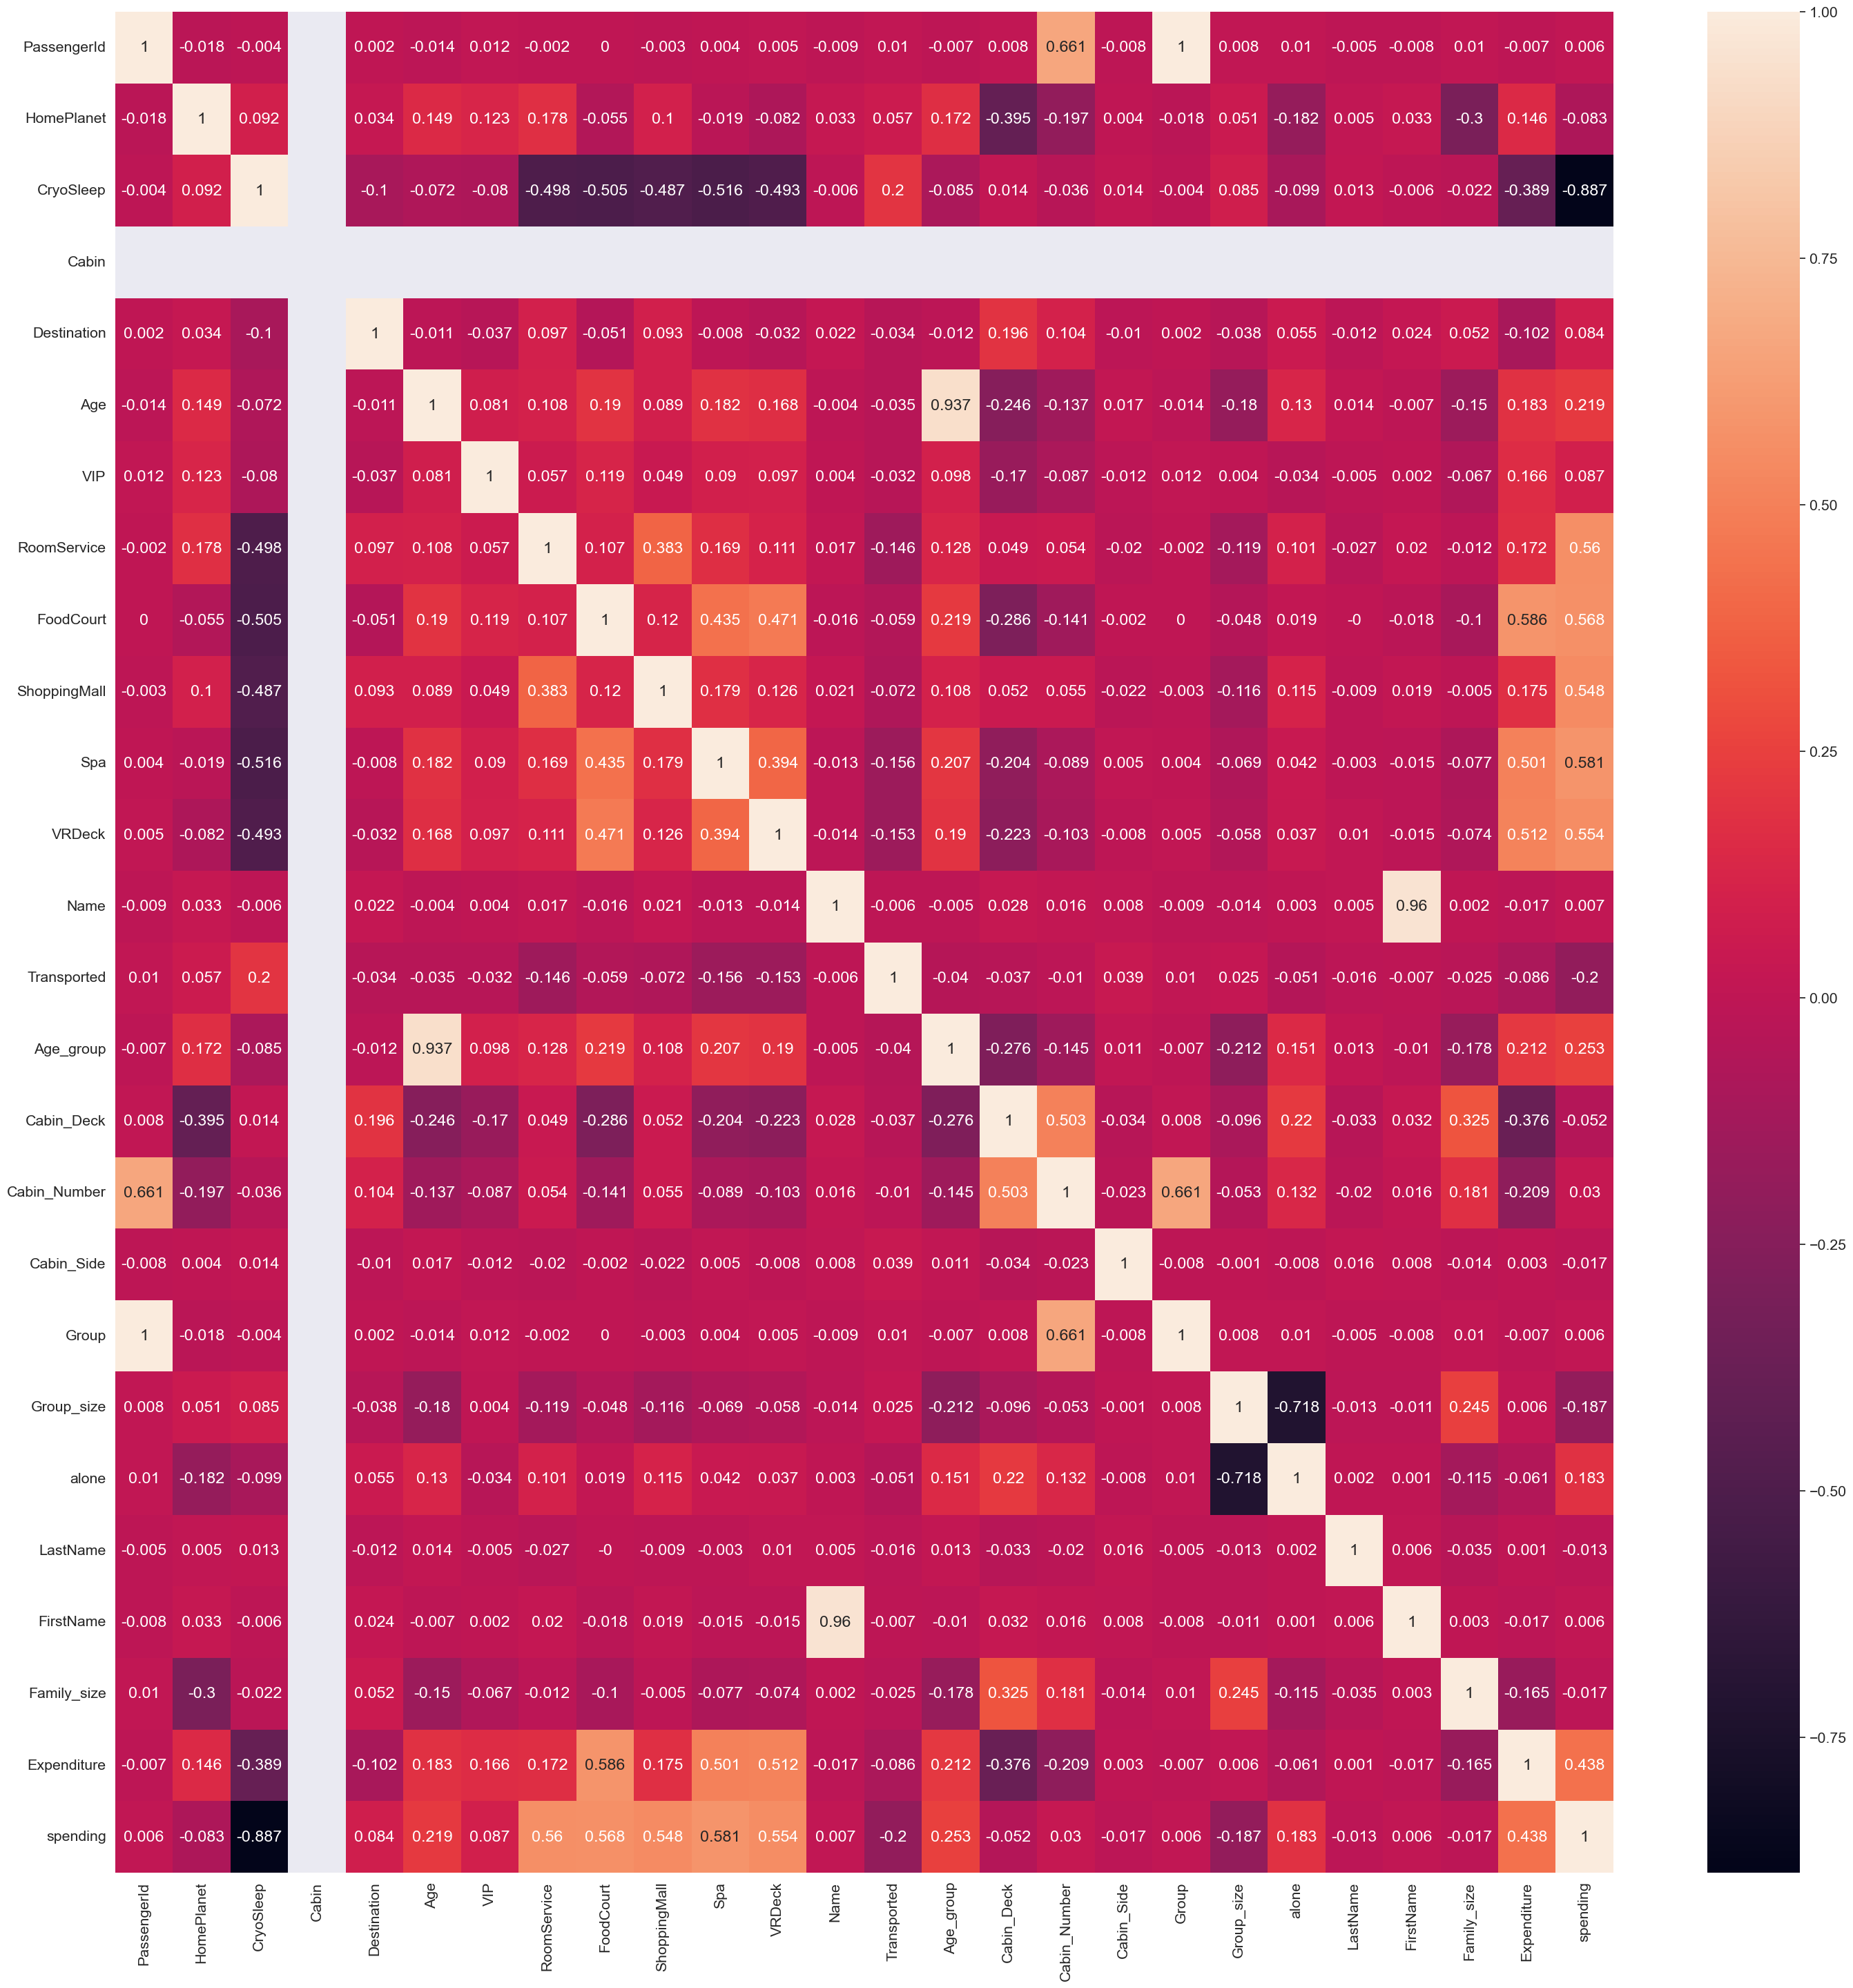
\includegraphics[scale=0.2]{Sec4_2.png}
                \caption{Pearson product-moment correlation coefficient}
            \end{figure}

            从图中可以看到PassengerId和Cabin\_Number有很强的正相关性,这是之前所没有发现的,因此虽然Cabin\_Number的缺失值填补方法使用的是random函数,依旧决定保留该特征。

            而HomePlanet正如之前分析的与Cabin\_Deck有较强的相关性;CryoSleep与五个消费特征,及spending,Expenditure特征相关性较强。

            Destination、Age、VIP三个特征和其他特征都没有较强的相关性,其中与Destination相关性最强的是Cabin\_Deck特征,符合之前的填补方法。

            五个消费特征除了与CryoSleep和spending、Expenditure特征相关性较强,互相也具有不同的相关性,这是之前填补时没有发现的趋势。

            让人比较意外的是,Family Size和LastName与Name特征相关性非常弱,而Family Size 和LastName之间相关性也较弱。
            

    \subsection{特征选择}

        首先基于之前分析过程中对于后续训练不需要的数据进行丢弃。丢弃了PassengerId,因为最有用的信息Group特征已经被重新构造;丢弃了Cabin特征,因为Cabin特征已经被重新构造,但保留了之前打算丢弃的Cabin\_Number特征,因为通过图31的皮尔森相关系数热力图可以发现,该特征与其他特征有着一定相关性,可以保留;
        丢弃了Name,First Name和Last Name,因为Last Name信息与Group高度重叠,而First Name的用处不大;丢弃了Group Size,因为Group Size 最重要的差别是Group中的乘客数量是否大于1,而这个差别可用特征Alone代替;
        丢弃了Family Size,因为该特征与Group Size高度重叠。

        最后保留的特征如图32所示。

        \begin{figure}[H]
            \centering
            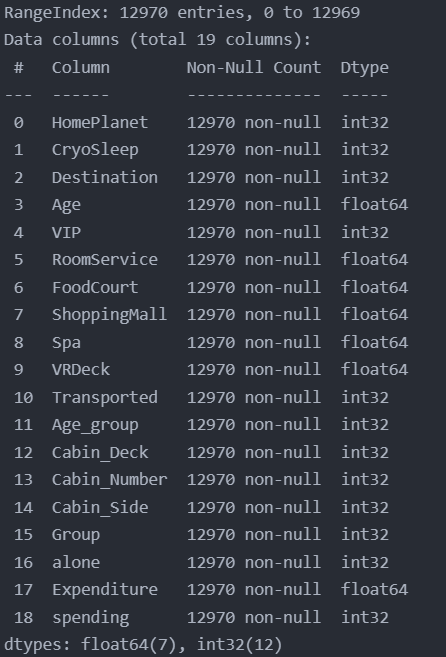
\includegraphics[scale=0.5]{Sec4_3.png}
            \caption{保留特征}
        \end{figure}

\end{document}